\section{Layout Transformations}\label{sec:transformations}

The layout-agnostic algorithms can benefit from performance gains that are achieved by choosing the best layout for given problem and architecture. However, in real-world scenarios, the layout of the input and output data structures is often prescribed as an inherent part of the algorithm interface, or even selected by the caller (in case of generic interfaces). Here, we show a straightforward way to generate code that transforms the code into the desired layout.


% -----------------------------------------------------------------------------
\subsection{Semi-automated transformation layer}
% -----------------------------------------------------------------------------

An abstract workflow of any data-processing program may be simplified to 3 phases --- \emph{loading} of the data into possible intermediate structures, \emph{execution} of the operation on the data, and \emph{storing} of the contents of possible intermediate structures into the target buffers.

To ensure optimal layout for the execution while keeping the input and output format as prescribed or selected by the caller, an adaptive layer can be introduced between steps 1--2, and 2--3 of the workflow. This layer would handle the transformation of the data from the original `external' input format into the optimal `internal` input format, and from optimal output format to the final output format. Assuming that the memory management in the second step is properly decoupled from array representation, the \emph{layout transformation} in the adaptive layers can be written as a generic routine using \Noarr{} library, as shown on an example for arrays with 2 indexes in Listing~\ref{lst:transform}.

\begin{listing}
    \vspace{-10pt}
    \inputmintedcpp{noarr/code-snippets/transform.cpp}
    \vspace{-20pt}
    \caption{Generic layout transformation routine for 2-index arrays.}
    \label{lst:transform}
\end{listing}

In the example, the transformation function (lines 1--7) operates on two \texttt{bag} structures, copying their contents element by element from a bag with data that use input layout to a bag with the desired layout, effectively performing the layout transformation. A helper function (lines 9--20) further simplifies the data transformation by determining if a layout change is really needed, and executing transformation (and copying the data) conditionally only in that case.

\begin{listing}
    \vspace{-10pt}
    \inputmintedcpp{noarr/code-snippets/matmul_transform.cpp}
    \vspace{-20pt}
    \caption{Outline of layout transformation layer for matrix multiplication example.}
    \label{lst:matmul_transform}
\end{listing}

These transformation routines may be readily used in other algorithms, as demonstrated in Listing~\ref{lst:matmul_transform} that wraps a matrix multiplication algorithm similar to the one from Listing~\ref{lst:matmul}.

We note that it is possible to implement the layout transformation function generically for any layout, for example by adapting the layout objects to work in range-based for-loops. Complex design considerations of the implementation (especially the static forwarding of the dimension identifiers) are however out of scope of the current \Noarr{} implementation.

% -----------------------------------------------------------------------------
\subsection{Exploring all layout combinations}
% -----------------------------------------------------------------------------

Given the possibility to work with arbitrary input and output layouts, we may expand the experiment from Section~\ref{sec:layouts-agnostic} to a larger spectrum of possible combinations of input and output layouts. We utilize the schema from Listing~\ref{lst:matmul_transform} to systematically loop through and benchmark all $6^3$ combinations of the layouts for the tiled matrix multiplication. The results are shown in Figure~\ref{fig:matmul_heatmap_all}.

\begin{figure}
	\centering
	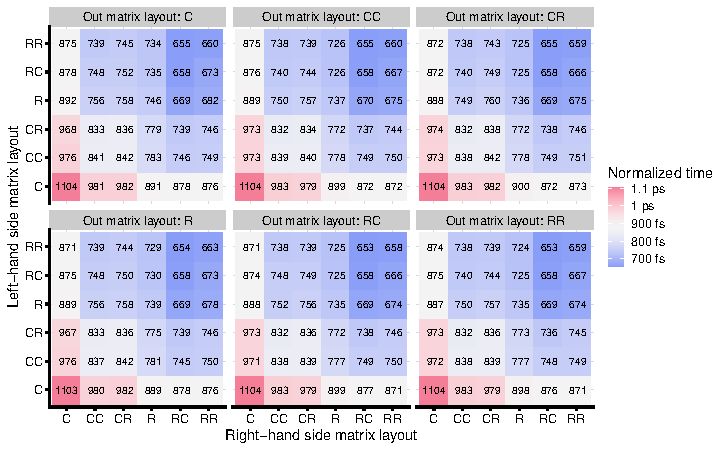
\includegraphics{plots/heatmap_all.pdf}
	\caption{Performance overview of layout combinations in matrix multiplication (X and Y axes represent the layout of right and left operand of the multiplication, layouts of the output are plotted separately). We report the normalized time per asymptotic operation, i.e., wall time divided by $N^3$.}
	\label{fig:matmul_heatmap_all}
\end{figure}

The results imply that the kernel performed best with $\textbf{RR}\times \textbf{RC}=\textbf{RR}$ layout combination, which was expected for tiled algorithm. The layout of input matrices turns out to be very important as the worst configuration ($\textbf{C}\times \textbf{C}$) is almost two times slower than the best one. On the other hand, the performance differences for the output matrix layouts are almost negligible. As in Section~\ref{sec:layouts-agnostic}, the main result is again methodological: The programmers may easily screen through all possible layouts for their data structures, and choose a reliable optimum for inclusion in production software.

% -----------------------------------------------------------------------------
\subsection{Transformation overhead}
% -----------------------------------------------------------------------------

While the algorithm performance is determined mainly by the layout combinations, the absolute performance differences are not huge. For example, the commonly used row-major format (i.e., $\textbf{R}\times \textbf{R} = \textbf{R}$) is only about 12\% slower on selected matrix sizes, which makes it at least competitive. We may therefore ask whether the data transformation overhead would not nullify the benefits of optimal layouts.

% The findings of this semi-automated layout transformation can in reasonably simple programmatic way show insights into the behavior of the specific function in terms of the memory access pattern and caches utilization. With minimal effort, this principle can be applied on multi-stage pipeline algorithms where each stage expects different memory layout for the most optimal computation. 

% However, a duration of the actual transformation needs to be accounted into as well. Depending on the layout pair to be transformed, the size of data and the actionable function, the duration of the transformation can sometimes diminish the performance gain resulted from the optimal layout usage in the selected algorithm. 

To clarify this concern, we have analyzed the layout transformation overhead for various matrix sizes and layouts. The key results are summarized in Figure~\ref{fig:matmul_comp}. We have observed that in the case of larger matrices ($N>10000$), the overhead is negligible, mostly because the asymptotic complexity difference between the transformation algorithm ($\mathcal{O}(N^2)$) and the multiplication ($\mathcal{O}(N^3)$). For smaller matrices (with $N$ around $1000$), the relative ratio of the transformation to computation time expectably increased. (Additionally, smaller matrices benefited more from caches, which make their layout slightly less important.) At that point, the baseline configuration $\textbf{R}\times\textbf{R}=\textbf{R}$ becomes the best option simply because it lacks the transformation overhead.

\begin{figure}
	\centering
	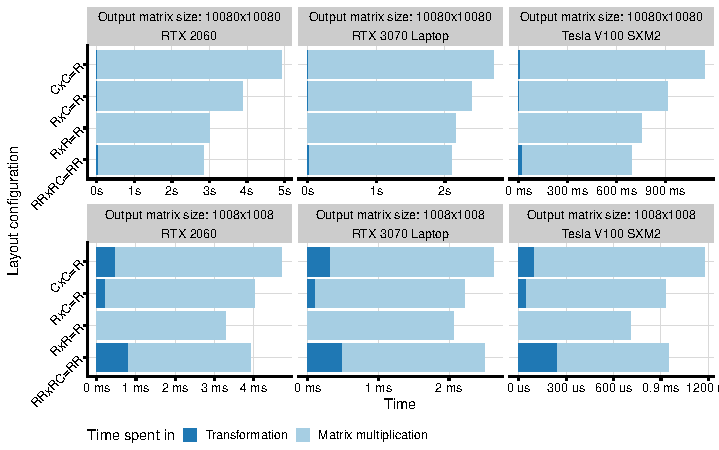
\includegraphics{plots/matmul_transform.pdf}
	\caption{Overhead of the layout transformation compared to actual time spent in the matrix multiplication algorithm. Only selected combinations of the layouts are shown for small and big matrix sizes.}
	\label{fig:matmul_comp}
\end{figure}

Finally, it is worth mentioning that the overhead of the transform algorithm can be reduced by selecting an appropriate copy-ordering for different layouts. The example in Listing~\ref{lst:transform} is designed as optimal for row-major layout, but it may not be optimal for other types of transforms. One of the objectives for the future research is to extract meta-information from the layout structures that would allow us to automatically select the optimal transform strategy (e.g., ordering of the nested for-loops).
